\documentclass[12pt]{report}
\usepackage[utf8]{inputenc}
\usepackage[british, slovene]{babel}
\usepackage{graphicx}
\usepackage{setspace}
\usepackage{mathptmx}
\usepackage{pdfpages}
\usepackage{setspace}
\usepackage{csquotes}
\usepackage{float}
\usepackage{notoccite}
\usepackage{helvet} % helvetica?
\usepackage{wrapfig}
\usepackage{multicol}
\usepackage{amssymb}
\usepackage{amsmath}
\usepackage{mathtools}
\usepackage{mathrsfs}
\usepackage[T1]{fontenc}% http://ctan.org/pkg/fontenc
\usepackage{tikz}
\usepackage{titlesec}
\usepackage{titletoc}
\usepackage{subcaption}
\usepackage{listings}
\usepackage[backend=biber, maxbibnames=99, sorting=none]{biblatex}
\addbibresource{bibliography.bib}
\usepackage{vegovatitle}
\usepackage[
        a4paper,% other options: a3paper, a5paper, etc
        left=3cm,
        right=2.5cm,
        top=2.5cm,
        bottom=2.5cm,
        % use vmargin=2cm to make vertical margins equal to 2cm.
        % us  hmargin=3cm to make horizontal margins equal to 3cm.
        % use margin=3cm to make all margins  equal to 3cm.
]{geometry}
\setlength{\parskip}{1em}
\DeclareQuoteAlias{croatian}{slovene}
%\renewcommand\thesection{\arabic{section}}
\setstretch{1.5}
\setlength{\parindent}{0pt}
\graphicspath{ {images/} }

% Format poglavij
\titleclass{\chapter}{straight}
\titleformat{\chapter}[hang]
{\normalfont\LARGE\bfseries}
{\LARGE\thechapter}
{0.5em}
{}
\titlespacing{\chapter}{0pt}{10pt}{10pt}

\lstset{tabsize=2, language=C++, breaklines=true, 
	breakatwhitespace=true,  xleftmargin=.1in}

\renewcommand{\lstlistingname}{Koda}

\title{KALKULATOR}
\project{Strokovno poročilo za 4. predmet splošne mature}
\author{Rok Strah, R 4. C}
\mentor{Darjan Toth, prof.}

\lstset{%
	frameround=single,%
	xleftmargin = \parindent%
}
%\usepackage{compsci}
\renewcommand{\familydefault}{\sfdefault}
%\fontfamily{phv}\selectfont
\newcommand{\wdot}{\textcolor{white}{.}}
\newcommand{\anglimp}[1]{angl.~\emph{#1}}
\newcommand{\angl}[1]{(\anglimp{#1})}
\newcommand{\odstavek}{\wdot \\ \wdot \qquad}
\newcommand{\codequote}[1]{\textquote{\texttt{#1}}}
\newcommand{\angokr}[2]{(okrajšano #1 iz \anglimp{#2})}
\newcommand{\group}[2]{\parbox{#1}{\setstretch{0.5}\vspace{5pt}\texttt{#2}\vspace{5pt}}}
\newenvironment{alignitemize}
{

\begin{tabular}{@{$\bullet$ }ll}
}{
\end{tabular}

}

\begin{document}

\maketitle

\setcounter{page}{2}
\chapter*{Povzetek}
	To poročilo predstavlja funkcionalnost in implementacijo programa StrahCalc.
	To je kalkulator, ki je poleg številskega računanja tudi zmožen simbolnega računanja in omejenega risanja grafov.
	Najprej poročilo opiše tehnologije in koncepte, ki so bili uporabljeni za izdelavo naloge.
	Opiše tudi nekaj specifičnih implementacij, nato pa še opiše sintakso jezika, ki ga kalkulator podpira.
\section*{Ključne besede}
	Kalkulator, Exprtk, Qt, AST, ARS, TRS, SRS, C++
\begin{otherlanguage}{british}
\chapter*{Abstract}
	This report describes the features and implementation of a calculator StrahCalc. 
	It also supports, along with numeric calculations, symbolic calculations and plotting graphs.
	The report first describes the technologies and concepts used for the project, then moves on to describe a few specific implementations.
	Lastly it describes the syntax of the language of the calculator.
\section*{Key words}
	Calculator, Exprtk, Qt, AST, ARS, TRS, SRS, C++
\end{otherlanguage}
\thispagestyle{empty}


{\pagestyle{empty}
\clearpage
\tableofcontents
\clearpage
\listoffigures
\clearpage}

\chapter{Uvod}
\label{intro}
	Za izdelavo kalkulatorja sem se odločil, ker mi je zelo všeč \textquote{Wolfram~Alpha}, vendar ni odprto-koden in se ga ne da razširjati.
	Zdelo se mi je, da bo to projekt, ki bo zahteval veliko načrtovanja, kar mi primanjkuje.
	Že na začetku, sem se odločil implementirati uporabniško definirane funkcije, ker je to res funkcionalnost, ki manjka v veliko drugih aplikacijah, ne le kalkulatorjih.
\chapter{Metodologija}
\label{methods}
	\section{Okolje, orodja, jezik in standardi}
		Za projekt sem uporabil programski jezik C++, razvojno orodje Qt Creator in nekaj knjižnic.
		\subsection{C++}
			C++ je Bjarne Stroustrup kot razširitev C-ju naredil v letu 1979.
			Želel je ustvariti učinkovit in prilagodljiv jezik podoben C-ju, ki pa bi tudi imel visoko-nivojske funkcije za organizacijo programa, kot so razredi.
			C++ je ISO/IEC JTC 1/SC 22/WG 21 standardizirala leta 1998, in od takrat so izdali 5 standardov:\\
			\parbox{\textwidth}{
			\begin{itemize}\setstretch{1.15}
				\item ISO/IEC 14882:1998\cite{cpp98} znan kot ISO C++ 1998 ali C++98 \cite{cpp_naming,cpp_ref,cpp_evolution},
				\item ISO/IEC 14882:2003\cite{cpp03} znan kot ISO C++ 2003 ali C++03 \cite{cpp_naming,cpp_ref,cpp_evolution},
				\item ISO/IEC 14882:2011\cite{cpp11} znan kot ISO C++ 2011, C++11 ali C++0x \cite{cpp_naming,cpp_ref,cpp_evolution},
				\item ISO/IEC 14882:2014\cite{cpp14} znan kot ISO C++ 2014, C++14 ali C++1y \cite{cpp_naming,cpp_ref,cpp_evolution} in
				\item ISO/IEC 14882:2017\cite{cpp17} znan kot ISO C++ 2017, C++17 ali C++1z \cite{cpp_naming,cpp_ref,cpp_evolution},
			\end{itemize}}
			sedaj pa delajo na naslednjem standardu, ki naj bi prišel v letu 2020 in je znan pod imenom C++20~\cite{cpp_naming,cpp_ref,cpp20_naming}.
			\odstavek
			Bjarne je leta 1979 začel razvijati \textquote{C with Classes}, razširitev C-ju in predhodnik C++.~\cite{cpp_evolution}
			Ko je delal na doktorski nalogi, je opazil, da ima jezik \textquote{Simula} nekaj funkcij, ki so zelo uporabne za velike projekte, toda je prepočasen za praktično rabo, vendar pa jeziku \textquote{BCPL}, ki je hiter, manjkajo visoko-nivojske funkcije za večje projekte.
			Med delom v \textquote{AT\&T Bell Labs} je bil navdihnjen izboljšati C s funkcijami podobnimi tistim v Simuli.
			Izbral si je C, ker je fleksibilen, učinkovit, dostopen in prenosljiv.
			Poleg vplivov C in Simule, so na C++ vplivali tudi drugi jeziki, kot so ALGOL 68, Ada, CLU in ML.
			Leta 1983 se je \textquote{C with Classes} preimenoval v C++, leta 1989 je pa bil dokončan C++ 2.0.
			\odstavek Bjarne je medtem tudi pisal knjigo \textquote{The C++ Programming Language}.
			Do sedaj je knjiga izšla v štirih izvodih v letih:~\cite{the_cpp_programming_language_wiki}\\
			\parbox{\textwidth}{
				\begin{itemize}\setstretch{1.15}
				\item 1985,
				\item 1991,
				\item 1997 in
				\item 2013
			\end{itemize}}
			ter v eni posebni izdaji leta 2000.
			Po C++ 2.0 se je C++ razvijal relativno počasi do 2011, ko je izšel standard C++11, ki je dodal veliko novih funkcij in je razširil \textquote{standard library} (okrajšano STL).
			Trenutno je C++, za Javo in C-jem, tretji najbolj znan programski jezik.~\cite{tiobe}
			\subsubsection{Filozofija C++}
				\begin{itemize}
					\item Splošna pravila:~\cite{cpp_evolution}
					\begin{itemize}
						\item Evolucijo C++ morejo voditi resnični problemi.
						\item Ne ukvarjaj se z nesmiselnim iskanjem popolnosti.
						\item C++ more biti uporaben zdaj.
						\item Vsaka funkcija jezika mora imeti razumno očitno implementacijo.
						\item Vedno zagotovi prehodno pot.
						\item C++ je jezik, ne popoln sistem.
						\item Zagotovi celovito podporo za vsak podprt slog.
						\item Ne poskušaj siliti ljudi, naj uporabljajo specifičen programski slog.
					\end{itemize}
					\item Pravila za podporo oblike:~\cite{cpp_evolution}
					\begin{itemize}
						\item Podpiraj smiselne oblikovne ideje.
						\item Zagotovi metode za organizacijo programa.
						\item Reči kar misliš.
						\item Vse funkcije morejo biti cenovno dostopne.
						\item Bolj je pomembno dovoliti uporabno funkcijo, kot pa preprečiti vsako zlorabo.
						\item Podpiraj sestavljanje programske opreme iz ločeno razvitih delov.
					\end{itemize}
					\item Jezikovno-tehnična pravila:~\cite{cpp_evolution}
					\begin{itemize}
						\item Nobenih implicitnih kršenj statičnega sistema tipov.
						\item Zagotovi tako dobro podporo za uporabniško-definirane tipe kot za vgrajene tipe.
						%\item \textquote{Locality} je dober.
						\item Izogibaj se zaporednih odvisnosti.
						\item Če si v dvomu, izberi varianto funkcije, ki jo je najlažje naučiti. % katero?
						\item Sintaksa je važna (ponavadi na čudne načine)
						\item Uporaba predprocesorja naj bi bila odpravljena.
					\end{itemize}
					\item Pravila za podporo nizko-nivojskega programiranja:~\cite{cpp_evolution}
					\begin{itemize}
						\item Uporabljaj tradicionalne (neumne) povezovalnike \angl{linker}.
						\item Nobenih neupravičenih nezdružljivosti s C.
						\item Ne pusti mesta za nizko-nivojski jezik pod C++ razen ASM.
						\item Za kar ne uporabljaš, ne plačaš \angl{zero-overhead~rule}.
						\item Če si v dvomu, zagotovi možnost za ročni nadzor.
					\end{itemize}
				\end{itemize}
		\subsection{Qt}
			Qt ([kjut] \anglimp{\textquote{cute}}~\cite{qt_pron}) je odprtokodno ogrodje za C++, ki ponuja razvojno okolje \textquote{Qt~Creator} \angokr{IDE}{Integrated~Development~Enviroment}, oblikovalec vmesnikov \textquote{Qt~Designer}, prevajalec \textquote{Qt~Linguist} in \textquote{Qt~Assistant}, ki kaže dokumentacijo in primere uporabe Qt knjižnic.
			V \textquote{Qt~Creator} imajo uporabniki na voljo tudi dostop do drugih treh programov.
			Qt knjižnice ločimo od drugih po njihovi predponi \textquote{\emph{Q}}--.
			Qt ima veliko funkcij, vendar najpomembnejše so pred-procesor moc~(iz~\anglimp{~Meta-Object~Compiler}~\cite{qt_moc}), Qt knjižnica gradnikov \angl{Qt Widgets} in Qt signali in reže \angl{Qt~Signals~\&~Slots}, s katerimi lahko nadziramo grafični vmesnik \angokr{GUI}{Graphical~User~Interface}.
			\subsubsection{Signali}
				Qt uporabnikom zagotavlja funkcije, za povezovanje signalov na reže.~\cite{qt_signals} To sta \codequote{connect} in \codequote{disconnect}.~\cite{qt_signals}
				Signali se ponavadi sprožijo, ko se objekt \angl{object} spremeni, pa bi to želeli sporočiti njegovemu staršu \angl{parent}.~\cite{qt_signals}
				Ko si signal sproži se ponavadi reže povezane nanj takoj izvedejo, kot navaden klic funkcije,~\cite{qt_signals}
				vendar pa če uporabljamo zaporedne povezave \angl{queued~connections} koda normalno nadaljuje z izvajanjem in se reže začnejo izvajati šele kasneje.~\cite{qt_signals}
			\subsubsection{Reže}
				Reže so navadne funkcije, na katere pa lahko povežemo signale.~\cite{qt_slots}
		\subsection{Knjižnice}
			\subsubsection{Exprtk}
				Exprtk je knjižnica za računanje za C++.~\cite{exprtk,exprtk_git}
			\subsubsection{KLFBackend}
				KLFBackend je C++ knjižnica, ki deluje kot vmesnik med aplikacijo in programom za izrisovanje \LaTeX{} kode.~\cite{qt_klf}
			\subsubsection{MufExprtkBackend}
				MufExprtkBackend je vmesnik med Qt programom in knjižnico Exprtk.
				Ker se ta knjižnica ne spreminja pogosto, jo lahko prevedemo posebej od aplikacije, kar skrajša čas prevajanja aplikacije za 1 do 10 minut, odvisno od zmogljivosti procesorja.
			\subsubsection{MufTranslate}
				MufTranslate je knjižnica, ki sem jo uporabil za prevajanje vmesnika v različne jezike.
				Za razliko od Qt Linguist knjižnica podpira prevode v obliki JSON datoteke.
		\subsection{Git}
			Git je sistem nadziranja verzij izvorne kode \angl{version~control~system}, ki se od ostalih takih sistemov odlikuje s svojo hitrostjo.~\cite{git}
			Git je ustvaril Linus Torvalds.
			Beseda \textquote{git} v britansko-angleškem slengu pomeni \textquote{neprijetna oseba}, Linus je pa ime razložil takole:~\cite{git_name}
			\begin{spacing}{0}
			\textquote{git} lahko pomeni karkoli, glede na tvoje razpoloženje.
			\begin{itemize}
				\item naključna kombinacija treh črk, ki jo je preprosto izgovoriti, vendar je ne dejansko uporablja noben pogost UNIX ukaz. Dejstvo, da je popačenka besede \textquote{get} je lahko, ali pa ne, povezano.
				\item neumen. zaničljiv in prezirajoč. preprost. Izberi si besedo iz slovarja slenga.
				\item \textquote{global~information~tracker}: si dobre volje in dejansko deluje za tvoje potrebe. Angeli pojejo in svetloba nenadoma zapolni prostor.
				\item \textquote{goddamn~idiotic~truckload~of~sh*t}: ko se pokvari 
			\end{itemize}
			\end{spacing}
		\subsection{\LaTeX}
			\LaTeX{} ([lateh] iz grško $\tau\epsilon\chi\nu\eta$) je izjemno močno programsko okolje za urejevanje (oblikovanje in izpis) besedil, ki ga je ustvaril znani ameriški matematik, računalnikar in programer Donald Knuth.
			Razširjen je na univerzah, še posebej se pa uporablja na področjih matematike, fizike in računalništva.
		\subsection{Linux}
			Linux je družina prostih in odprto-kodnih operacijskih sistemov, ki za jedro \angl{kernel} uporabljajo \textquote{Linux}.
			Aplikacijo sem začel razvijati na Windows operacijskem sistemu, vendar sem moral zaradi omejitev sistema zamenjati na Linux. %TODO: expand?
		\subsection{Druga orodja in standardi}
			\subsubsection{AStyle}
				AStyle je program, ki samodejno oblikuje izvorno kodo po definiciji, ki jo podaš.~\cite{astyle}
				Qt tudi omogoča povezavo z AStyle preko dodatkov \angl{plugin}.
			\subsubsection{CMake}
				CMake je prosta in odprto-kodna rešitev za avtomatizacijo grajenja projektov.~\cite{cmake}
				V primerjavi s Qt-ovim qmake je močnejši, vendar zahtevnejši za uporabo.
			\subsubsection{Ninja}
				Ninja je prost odprto-kodni sistem za grajenje projektov.~\cite{ninja}
				Za razliko od ostalih takih sistemov je bistveno hitrejši.~\cite{ninja}
				Čeprav ga je možno uporabljati samega, je mišljeno, da se ga uporablja v povezavi z programom, ki generira \codequote{.ninja} datoteke, kot je CMake.~\cite{ninja}
			\subsubsection{Clang}
				Clang je prost odprto-kodni vmesnik za jezike družine C, ki se od GCC-ja razlikuje predvsem po boljših sporočilih in hitrosti.~\cite{clang}
			\subsubsection{JSON}
				JSON (iz \anglimp{JavaScript~Object~Notation}) je način zapisa tabel in objektov v tekstovno datoteko.~\cite{json}\\
				{Struktura JSON:~\cite{json}
				\begin{itemize}\setstretch{1.15}
					\item JSON dokument je sestavljen iz objekta ali tabele.
					\item JSON objekt (slika \ref{fig:json_obj}) je sestavljen iz parov ključev in vrednosti.
					\item JSON tabela (slika \ref{fig:json_arr}) vsebuje več vrednosti.
					\item Ključ je niz(slika \ref{fig:json_str}), vrednost (slika \ref{fig:json_val}) je pa lahko niz , število (slika \ref{fig:json_num}), tabela, objekt, dvojiška vrednost (true in false) ali null.
				\end{itemize}}
			\begin{figure}[H]
				\centering
				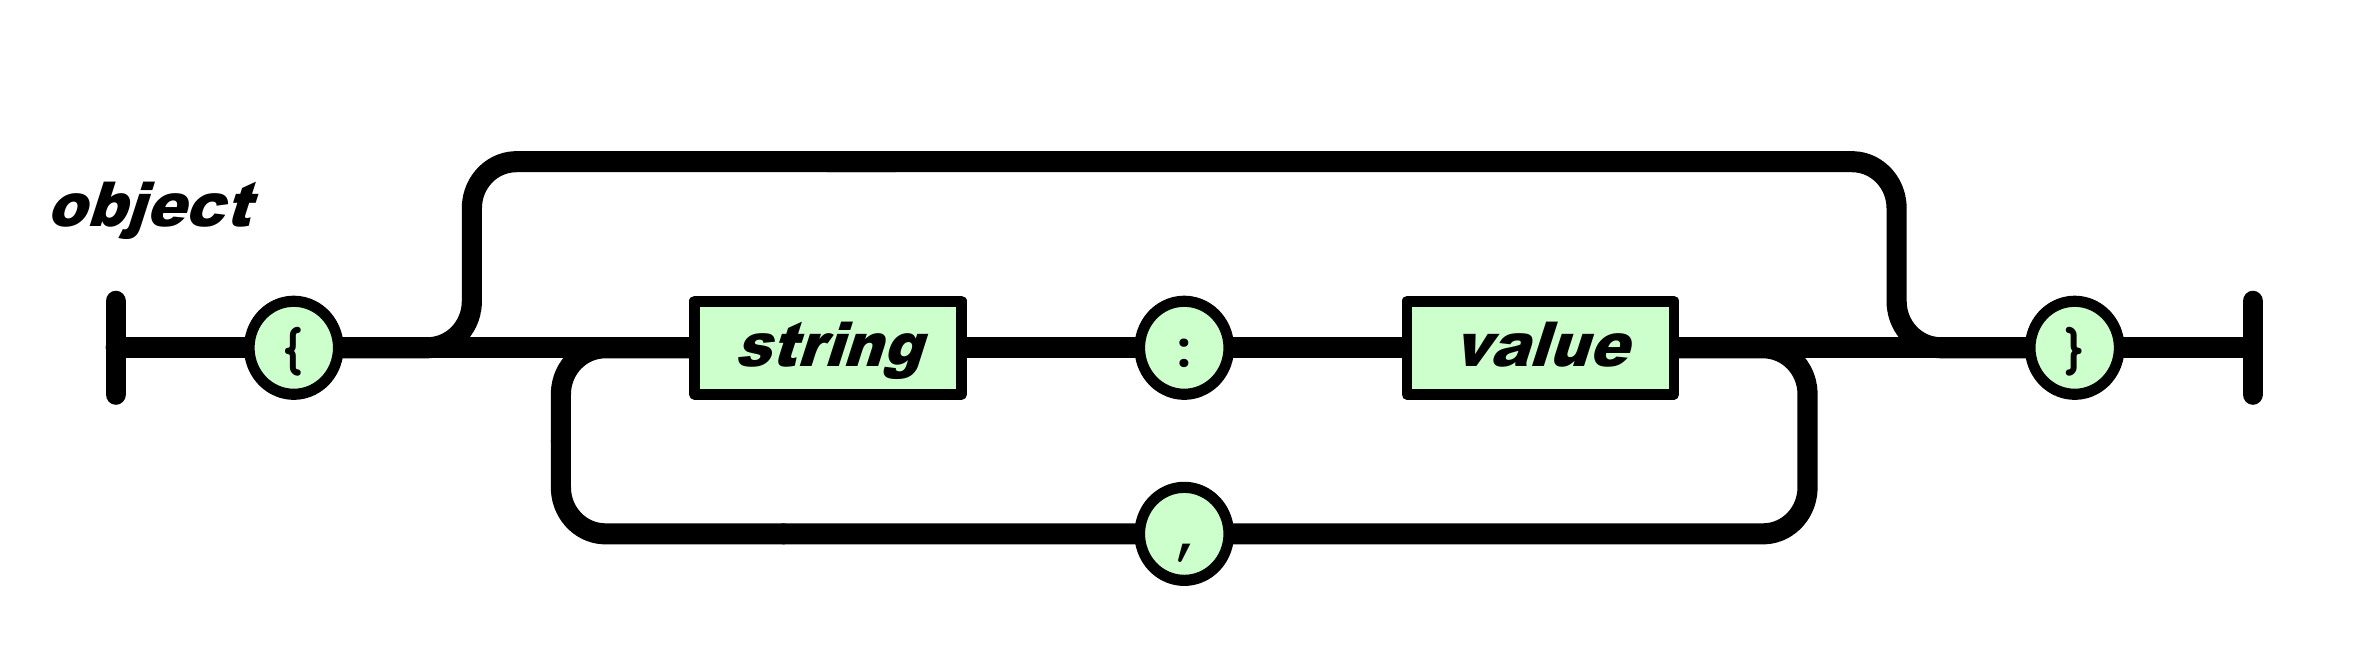
\includegraphics[width=\textwidth]{json_object.png}
				\caption{JSON objekt~\cite{ecma404}}
				\label{fig:json_obj}
			\end{figure}
			\begin{figure}[H]
				\centering
				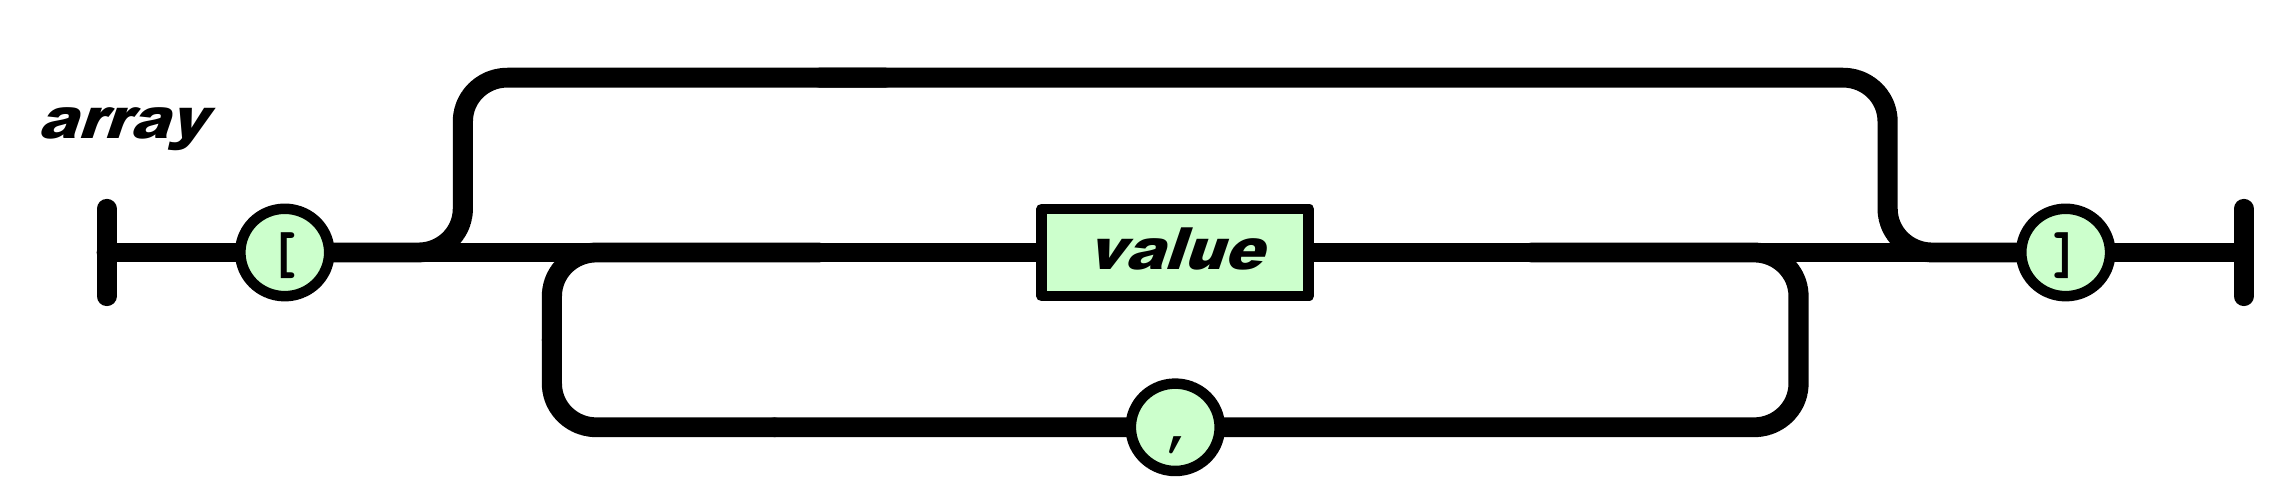
\includegraphics[width=\textwidth]{json_array.png}
				\caption{JSON tabela~\cite{ecma404}}
				\label{fig:json_arr}
			\end{figure}
			\begin{figure}[H]
				\centering
				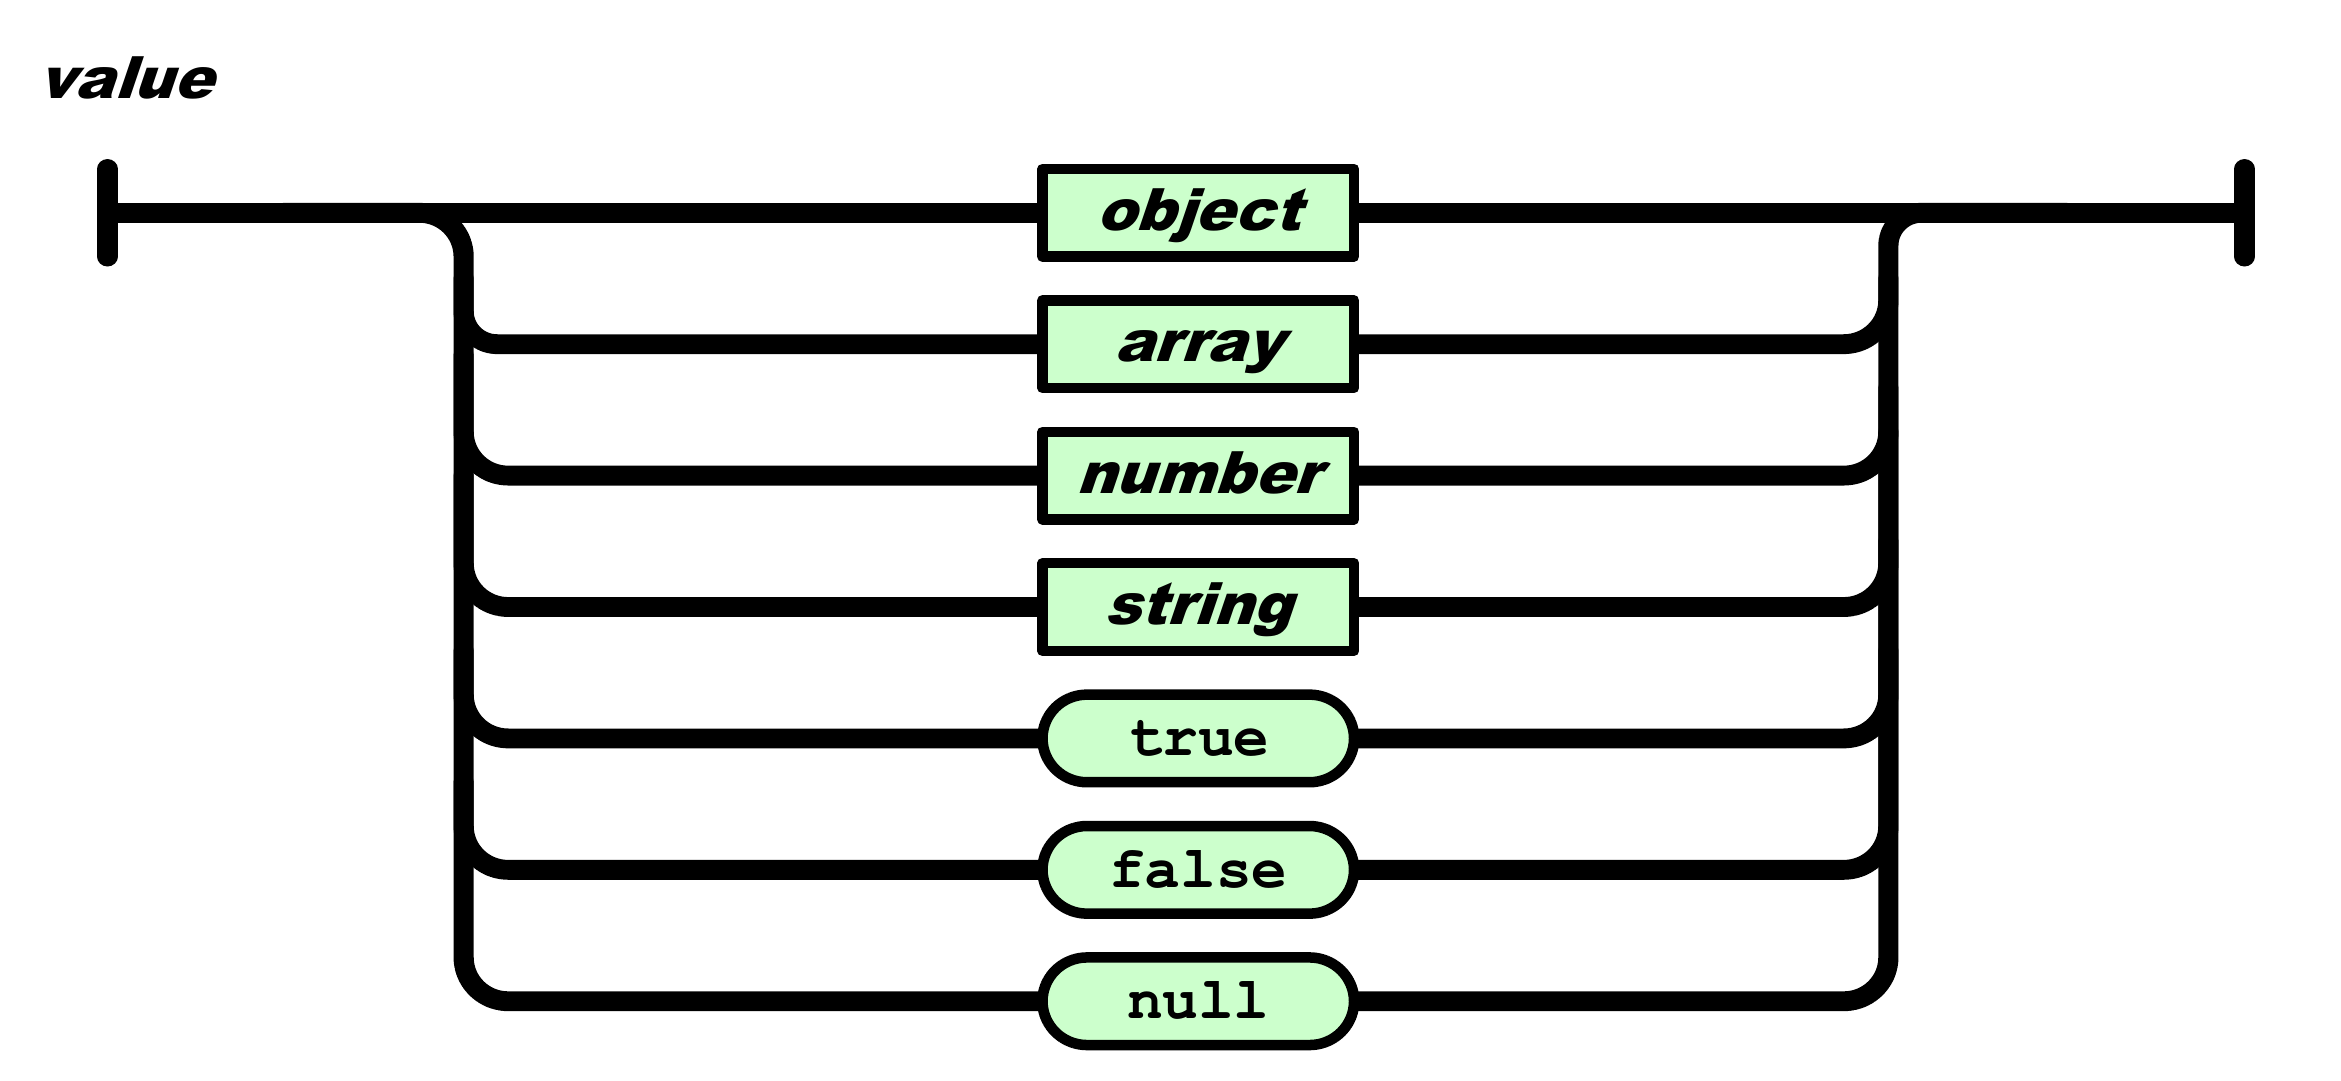
\includegraphics[width=\textwidth]{json_value.png}
				\caption{JSON vrednost~\cite{ecma404}}
				\label{fig:json_val}
			\end{figure}
			\begin{figure}[H]
				\centering
				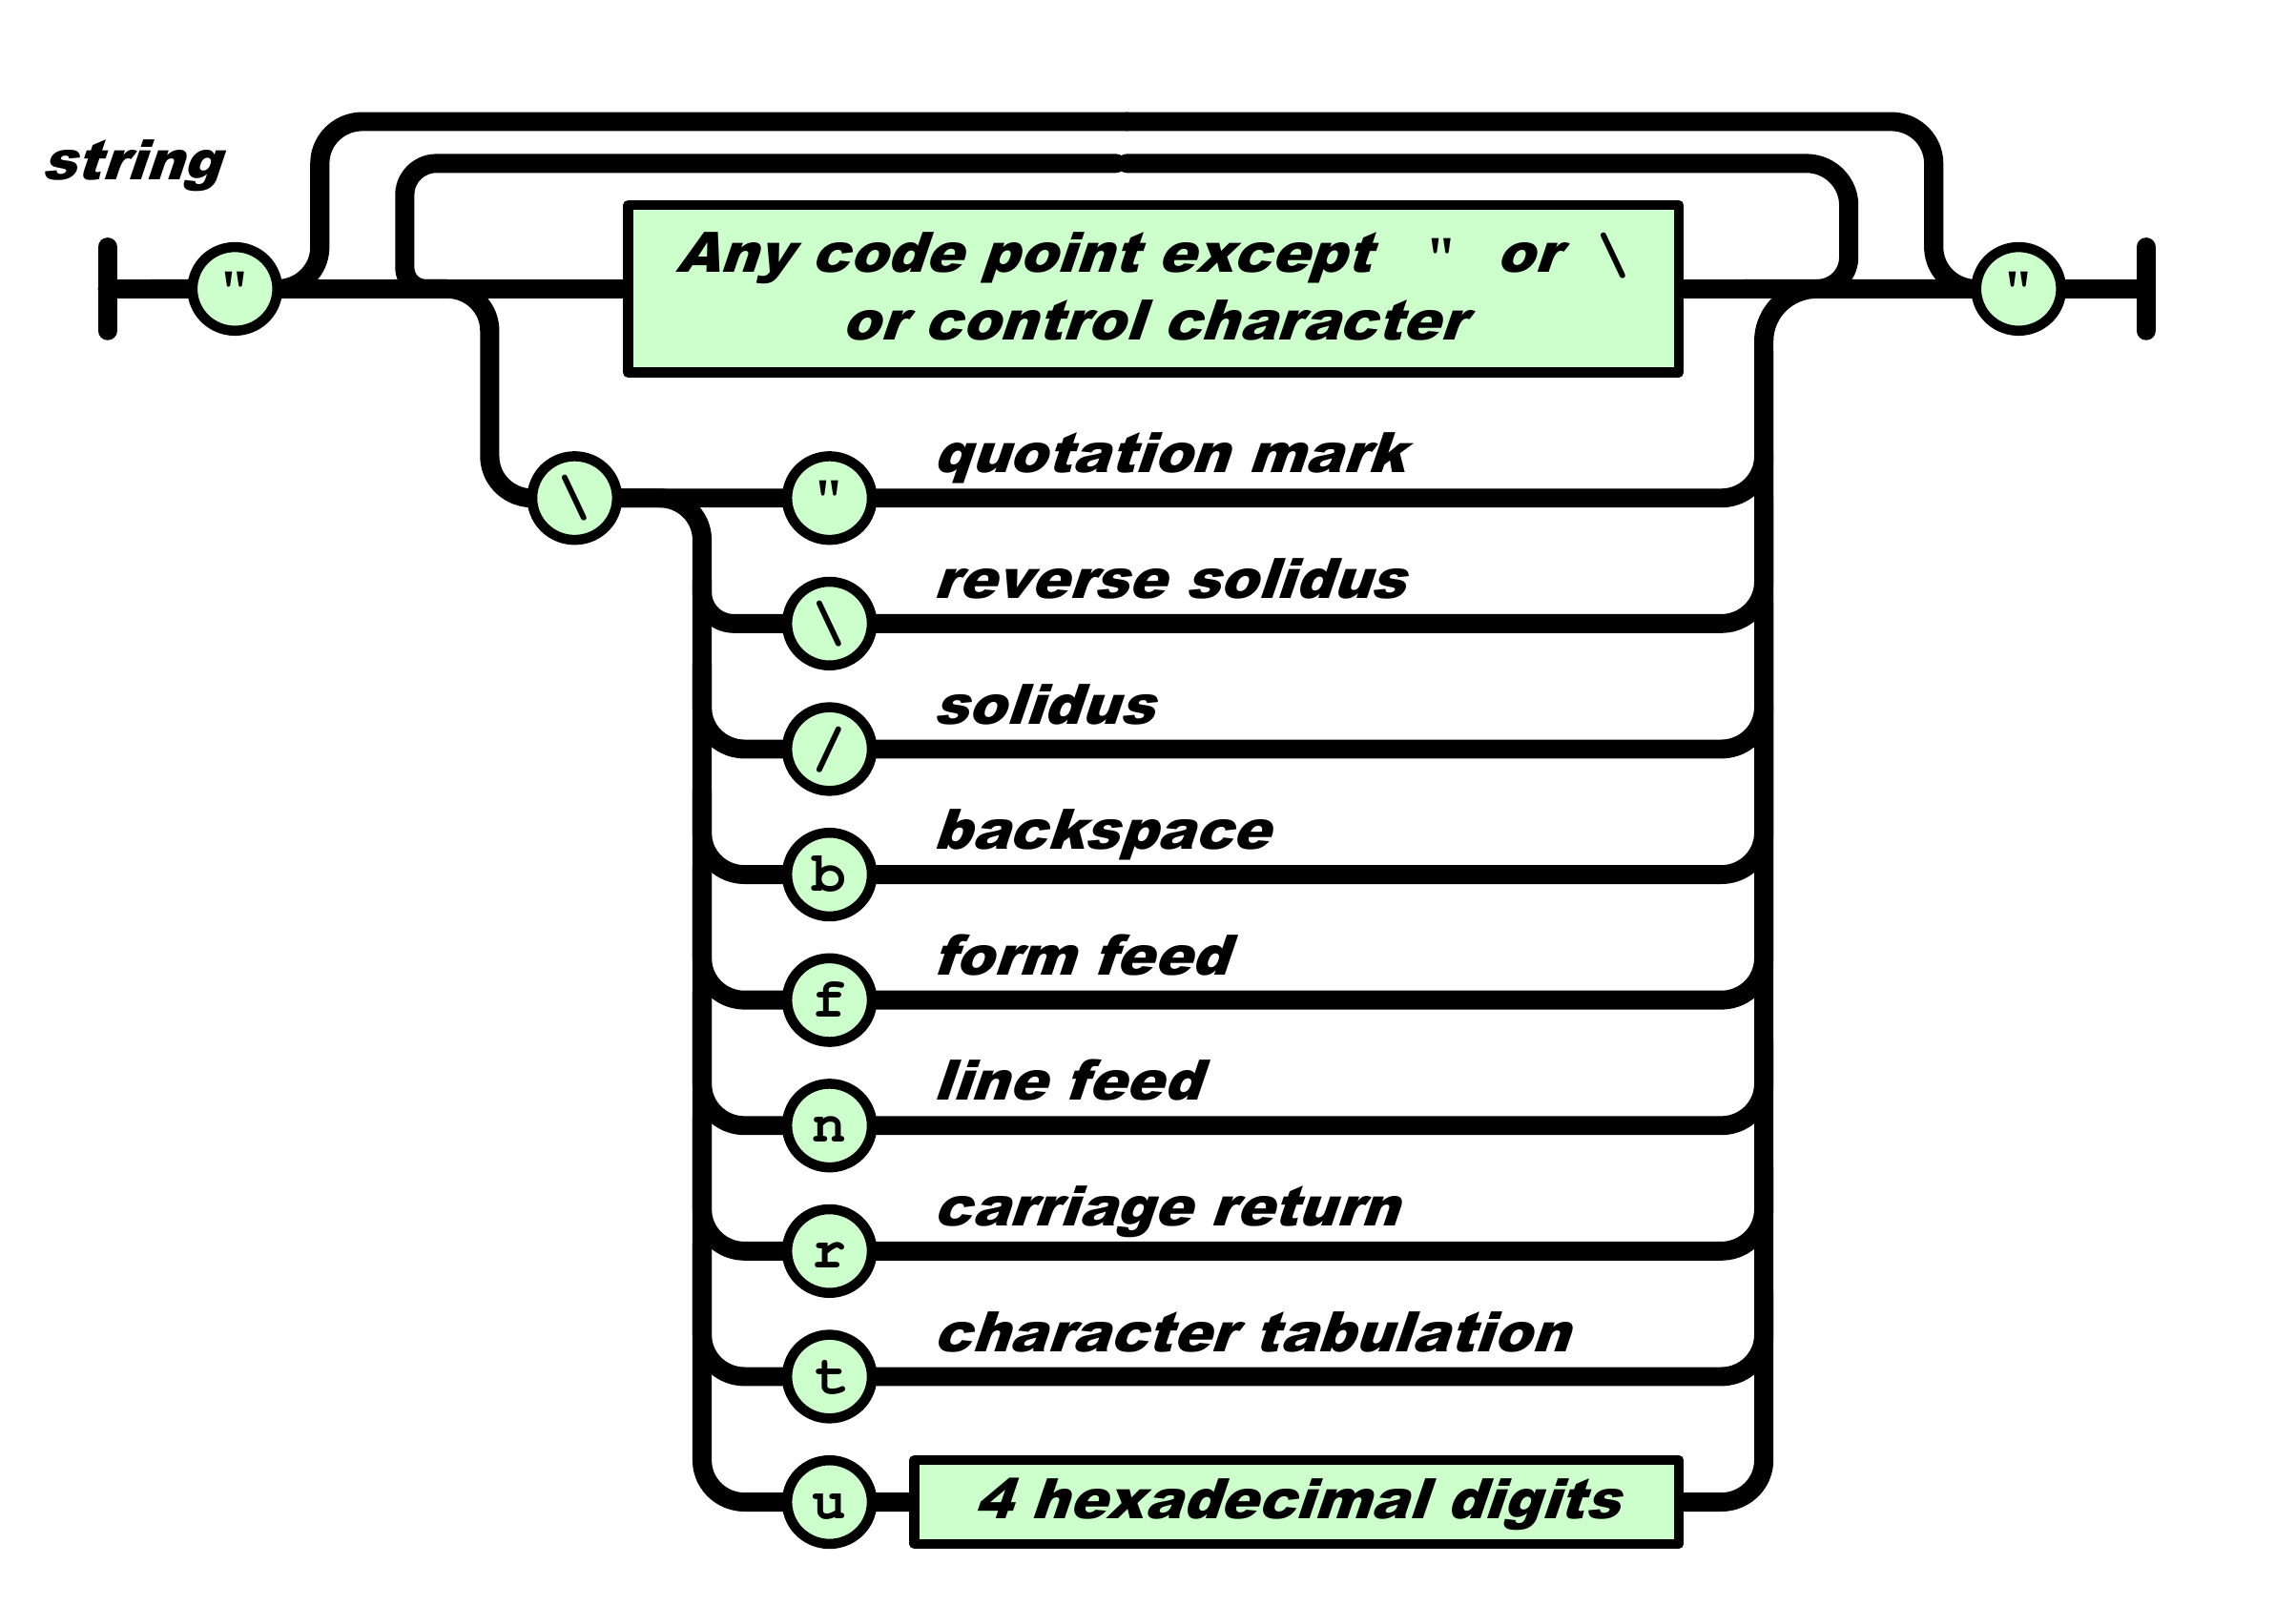
\includegraphics[width=\textwidth]{json_string.png}
				\caption{Niz v JSON~\cite{ecma404}}
				\label{fig:json_str}
			\end{figure}
			\begin{figure}[H]
				\centering
				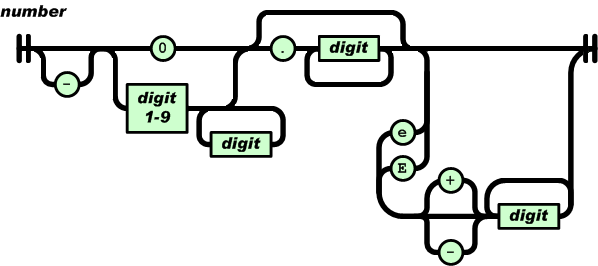
\includegraphics[width=\textwidth]{json_number.png}
				\caption{Število v JSON~\cite{ecma404}}
				\label{fig:json_num}
			\end{figure}
	\section{Koncepti} % TODO: translate
		\subsection{Abstrakten sistem prepisovanja}
			Abstrakten sistem prepisovanja \angokr{ARS}{abstract rewriting system} je množica objektov $A$ in binarna relacija, ki pove kako preoblikovati te objekte.
			To binarno relacijo imenujemo \textquote{prepisovalna relacija}~\cite[p.~7]{terese} in jo dobimo iz množice pravil.
			ARS se uporabljajo na več področjih, npr. v matematiki, računalništvu, logiki in jezikoslovju.
		\subsection{Sistem prepisovanja členov}
			Sistem prepisovanja členov \angokr{TRS}{term rewriting system} je ARS, ki ima za elemente člene matematičnega izraza.
		\subsection{Sistem prepisovanja nizov}
			Sistem prepisovanja nizov \angokr{SRS}{string rewriting system} ali semi-Thue sistem je ARS, ki ima za elemente nize ali podnize.
		\subsection{Abstraktno sintaktično drevo}
			Aplikacija iz vnosa zgradi abstraktno sintaktično drevo \angokr{AST}{abstract syntax tree}.
			Ko je AST zgrajen, omogoča implementacijo TRS za poenostavljanje izrazov in SRS za pretvarjanje izraza v sintakso jezika \LaTeX{}.
\chapter{Funkcionalnost}
\label{features}
	\section{Glavno okno}
	\label{mainwindow}
		\parbox{\textwidth}{
		Na glavnem oknu je več zavihkov~(glej~sliko~\ref{fig:mw_tabs}) ---
		\textquote{Kalkulator}, \textquote{Napredno}, \textquote{Grafično}, \textquote{Spremenljivke}, \textquote{Konstante} in \textquote{Zgodovina}
		--- vsak s svojo funkcijo.
		\begin{figure}[H]
			\centering
			
\includegraphics{mw_tabs.png}
			\caption{Zavihki na glavnem oknu}
			\label{fig:mw_tabs}
		\end{figure}.}
		\parbox{\textwidth}{
		V zgornjem meniju najdemo nekaj orodji~(glej~sliko~\ref{fig:tools}) , kot npr. \textquote{Nastavitve} ali \textquote{O programu}
		\begin{figure}[H]
			\centering
			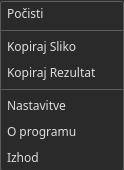
\includegraphics{tools.png}
			\caption{Orodja v zgornjem meniju}
			\label{fig:tools}
		\end{figure}}
		\parbox{\textwidth}{
		Na dnu je pa tudi viden status aplikacije~(glej~sliko~\ref{fig:mw_status}), ki sporoča uporabniku, kaj aplikacija trenutno dela.
		\begin{figure}[H]
			\centering
			
\includegraphics{mw_status.png}
			\caption{Trenutni status aplikacije}
			\label{fig:mw_status}
		\end{figure}}
		\parbox{\textwidth}{
		\subsection{Kalkulator}
			Prvi zavihek je \textquote{preprost} kalkulator.
			Zgoraj je vrstica za vnos računa, pod njo so pa trije gumbi, dva za kopiranje rezultata in en za začetek računanja.
			Računati začne tudi ob pritisku tipke \textquote{Enter}.
			Celoten zavihek s primerom zgleda takole:
			\begin{figure}[H]
				\centering
				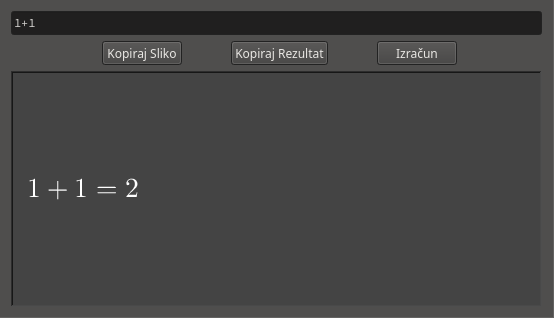
\includegraphics{mw_calc.png}
				\caption{Preprost kalkulator}
				\label{fig:mw_calc}
			\end{figure}}
		\parbox{\textwidth}{
		\subsection{Napredno}
			Napredni kalkulator je razširitev preprostega kalkulatorja.
			Vnosno polje za račun dovoljuje vnašanje večih vrstic, kar pomeni, da je možno uporabiti tudi kompleksnejše strukture kot so zanke ter pogojni stavki.
			Poleg rezultata se pa tudi izriše poenostavljen izraz.
			Celoten zavihek s primerom zgleda takole:
			\begin{figure}[H]
				\centering
				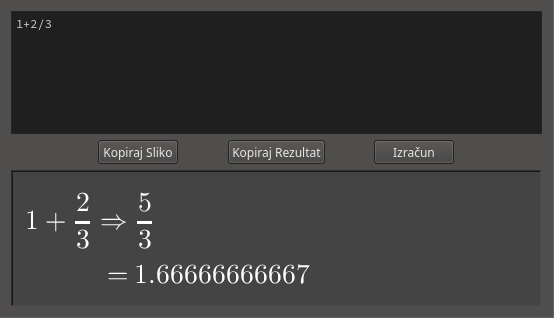
\includegraphics{mw_adv.png}
				\caption{Napredni kalkulator}
				\label{fig:mw_adv}
			\end{figure}}
		\parbox{\textwidth}{
		\subsection{Grafično}
			Vnosno polje je podobno kot v naprednem kalkulatorju, manjka pa gumb \textquote{Kopiraj rezultat}, saj aplikacija v tem načinu nič ne računa, ampak riše grafe funkcij, ki jih pišemo v vnosno polje.
			Celoten zavihek s primerom zgleda takole:
			\begin{figure}[H]
				\centering
				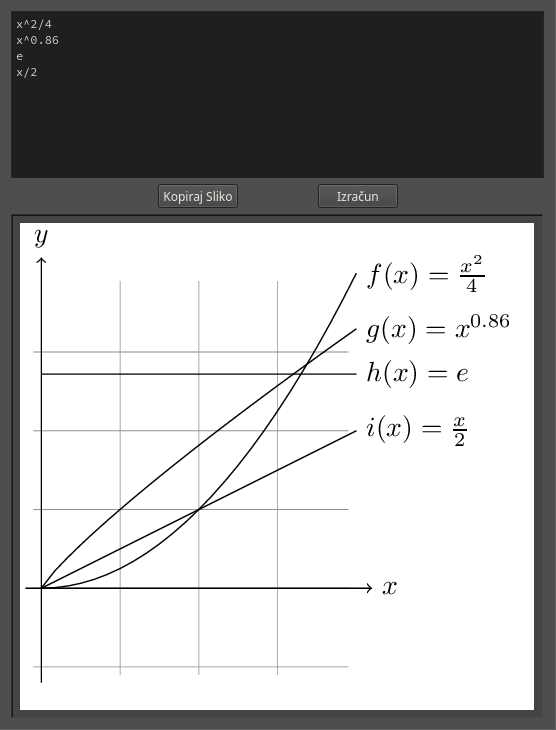
\includegraphics[height=550px]{mw_plot.png}
				\caption{Grafični kalkulator}
				\label{fig:mw_plot}
			\end{figure}}
		\parbox{\textwidth}{
		\subsection{Spremenljivke in Konstante}
			Ta dva zavihka v tabeli prikazujeta vse spremenljivke in konstante, ki so vnesene v programu.
			Celoten zavihek s primerom zgleda takole:
			\begin{figure}[H]
				\centering
				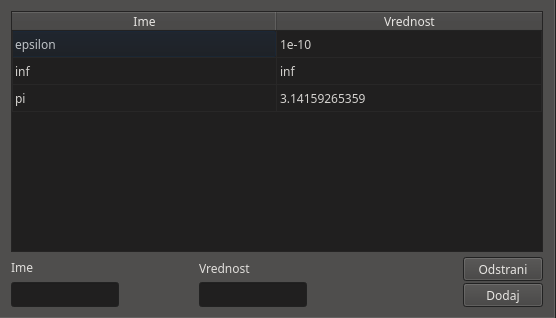
\includegraphics[height=230px]{mw_const.png}
				\caption{Konstante}
				\label{fig:mw_const}
			\end{figure}}
		\parbox{\textwidth}{
			\subsection{Zgodovina}
			Aplikacija beleži zgodovino vnesenih računov.
			Celoten zavihek s primerom zgleda takole:
			\begin{figure}[H]
				\centering
				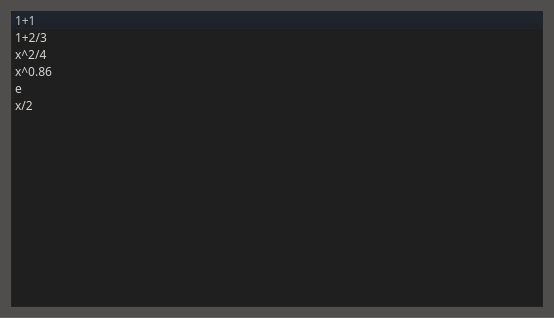
\includegraphics[height=230px]{mw_hist.png}
				\caption{Zgodovina}
				\label{fig:mw_hist}
			\end{figure}}
	\parbox{\textwidth}{
	\section{Nastavitve}
		V nastavitvah lahko nastavljamo jezik, čas prikaza statusa, velikost izrisane slike in barvo slike, lahko pa tudi vklopimo in izklopimo razne funkcije.
		Celotno okno s privzetimi nastavitvami zgleda takole:
		\begin{figure}[H]
			\centering
			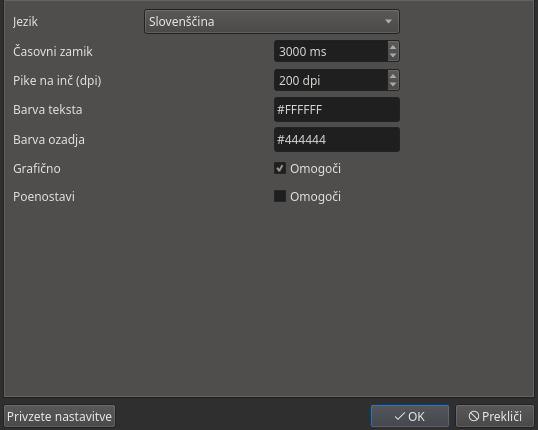
\includegraphics{settings.png}
			\caption{Nastavitve}
			\label{fig:settings}
		\end{figure}
		Na dnu okna najdemo gumba \textquote{OK} in \textquote{Prekliči} ter gumb za nastavitev privzetih vrednosti.}
	\section{Simboli}
	\label{symbol}
		%Aplikacija podpira simbolično računanje s pomočjo AST. % TODO: insert exprtree img
		Aplikacija iz podanega izraza zgradi AST, kar pa reši dva od problemov naloge.
			\subsection{Poenostavljanje izrazov}
				Poenostavljanje izrazov poteka v treh delih:
				\begin{itemize}
					\item ponovno poenostavljanje po preprostih pravilih,
					\item pretvorbe vseh elementov drevesa v ulomke in
					\item ponovno poenostavljanje po preprostih pravilih.
				\end{itemize}
				Prvi del poenostavi izraze kot so $ x + 0 $ in $ x^1 $, drugi del pretvori izraze kot so $ \frac{a}{b} + \frac{c}{d} $ v $ \frac{ad + bc}{bd} $ ali $ 1 + \frac{2}{3} $ v $ \frac{5}{3} $, tretji del pa poenostavi izraze oblike $ \frac{x}{1} $
			\subsection{Pretvorba v \LaTeX{}}
				Za pretvorbo v \LaTeX{} se program preprosto spusti po drevesu in na primer za ulomke izpiše \texttt{\{\textbackslash frac\{števec\}\{imenovalec\}\}}. Z le par preprostimi pravili dokaj zanesljivo prepiše cel izraz.
\clearpage			
\chapter{Implementacija}
\label{impl}
	\section{Drevesna struktura programa}
	\label{project_tree}
		\begin{wrapfigure}{r}{0.36\textwidth}
			\vspace{-45pt}
			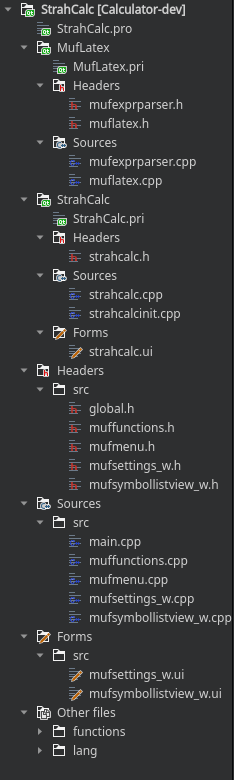
\includegraphics[width=160pt]{project_tree.png}
			\caption{Drevesna struktura programa}
			\label{fig:project_tree}
		\end{wrapfigure}
		\parbox{250pt}{
			\setstretch{0}
			Kot vidimo na sliki \ref{fig:project_tree} je projekt razdeljen na dva podprojekta:
			\begin{enumerate}
				\item StrahCalc in
				\item MufLatex,
			\end{enumerate}
		}\\
		\parbox{250pt}{
			\setstretch{0}
			ter dve skupini:
			\begin{enumerate}
				\item StrahCalc in
				\item MufLatex,
			\end{enumerate}
		}\\
		v drevesu je pa vključena še izvorna koda knjižnic, ki sem jih uporabil.
		Kot podprojekt \textquote{lang} sem dodal tudi jezikovne datoteke (za \codequote{MufTranslate}), kar je pospešilo prevajanje uporabniškega vmesnika.
		\subsection{StrahCalc}
		\label{tree_strahcalc}
			\parbox{250pt}{
				V podprojektu StrahCalc se nahajajo datoteke:
				\begin{enumerate}
					\setstretch{0}
					\item \textbf{global.h},
					\item \textbf{strahcalc.h},
					\item \textbf{strahcalc.cpp} in
					\item \textbf{strahcalcinit.cpp}.
				\end{enumerate}
			}\\
			V \textbf{strahcalc.h} je deklaracija razreda \codequote{StrahCalc}, ki deduje \codequote{QMainWindow} in nadzoruje glavno okno aplikacije, v \textbf{strahcalc.cpp} se pa nahaja definicija tega razreda, v \textbf{strahcalcinit.cpp} pa definicije funkcij za inicializacijo opisanih v razdelku \ref{constructor}.
			V ta podprojekt sem dodal \textbf{global.h}, v katerem se nahajajo funkcije, definicije in objekti, ki jih uporabljam v več datotekah.
		\clearpage
		\subsection{MufLatex}
		\label{tree_muflatex}
			\parbox{\textwidth}{
				V podprojektu MufLatex se nahajajo datoteke:
				\begin{enumerate}
					\setstretch{0}
					\item \textbf{mufexprparser.h},
					\item \textbf{mufexprparser.cpp},
					\item \textbf{muflatex.h} in
					\item \textbf{muflatex.cpp}.
				\end{enumerate}
			}\\
			Datoteka \textbf{mufexprparser.h} vsebuje deklaracijo razreda \codequote{MufExprParser}, ki je definiran v \textbf{mufexprparser.cpp}.
			V datoteki \textbf{muflatex.h} je deklaracija razreda \codequote{MufLatex}, ta ima pa definicijo v \textbf{muflatex.cpp}.
		\subsection{Headers}
		\label{tree_headers}
			\parbox{\textwidth}{
				V skupini Headers se nahajajo datoteke:
				\begin{enumerate}
					\setstretch{0}
					\item \textbf{muffunctions.h},
					\item \textbf{mufmenu.h},
					\item \textbf{mufsettings\_w.h} in
					\item \textbf{mufsymbollistview\_w.h},
				\end{enumerate}
			}\\
			\parbox{\textwidth}{
				ki deklarirajo manjše razrede:
				\begin{enumerate}
					\setstretch{0}
					\item \codequote{MufFuncions}, ki skrbi za dodajanje uporabniških funkcij iz datotek,
					\item \codequote{MufMenu}, ki skrbi za gornji meni,
					\item \codequote{MufSettings\_w}, ki skrbi za okno z nastavitvami in
					\item \codequote{MufSymbolListView\_w}, ki skrbi za prikaz spremenljivk in konstant v glavnem oknu.
				\end{enumerate}
			}
		\subsection{Sources}
		\label{tree_sources}
			\parbox{\textwidth}{
				V skupini Sources se pa nahajajo datoteke z definicijami razredov opisanih v razdelku \ref{tree_headers}:
				\begin{enumerate}
					\setstretch{0}
					\item \textbf{muffunctions.cpp},
					\item \textbf{mufmenu.cpp},
					\item \textbf{mufsettings\_w.cpp} in
					\item \textbf{mufsymbollistview\_w.cpp}.
				\end{enumerate}
			}
	\section{Glavno okno}
	\label{mainwindow_impl}
		\subsection{Inicializacija}
		\label{constructor}
			Aplikacija najprej naloži nastavitve in postavi par spremenljivk na začetne vrednosti, nato pa začne klicati podprograme za inicializacijo posameznih logičnih enot. % TODO: rewrite
			Potem poveže signal, ki se sproži, ko je rezultat obdelan, na režo, ki rezultat posreduje izrisovalcu.
			Na koncu še vpiše ves tekst v aplikacijo.
			\subsubsection{KLFBackend}
				Podprogram najde nastavitve \LaTeX{} ozadja in z njimi naredi nov \codequote{KLFPreviewBuilderThread}. % TODO: retranslate backend
			\subsubsection{Exprtk}
				Podprogram naredi nov \codequote{MufExprtkBackend} in poveže signal za konec računanja in signal za napake na njihove reže.
			\subsubsection{Glavno okno}
				Podprogram najprej kliče podprogram za inicializacijo gornjega menija in poskrbi, da ko se spremeni jezik v knjižnici za prevajanje, se tudi posodobi tekst.
			\subsubsection{Meni}
				Podprogram naredi nov \codequote{MufMenu} in poveže elemente menija na reže, ki bojo izvedle želeno akcijo.
			\subsubsection{Spremenljivke in konstante}
				Podprogram naredi nove \codequote{MufSymbolListView\_w}-je, jih doda v njihove zavihke, jih posodobi s podatki iz \codequote{Exprtk}-ja in poveže gumbe za dodajanje in odstranjevanje spremenljivk in konstant.
			\subsubsection{Funkcije}
				Podprogram najde pot do definicij funkcij in s to potjo naredi nov \codequote{MufFunctions}.
			\subsubsection{Kalkulator}
				Vsi trije podprogrami za inicializacijo zavihkov s kalkulatorji povežejo signale, ki sprožijo računanje na reže, ki začnejo računanje in povežejo gumbe za kopiranje rezultata.
				Nato nastavijo še kazalec na vnosno polje.
			\subsubsection{Nastavitve}
				Podprogram naredi nov \codequote{MufSettings\_w}.
				Nato najde pot do jezikovnih datotek in jezike doda v spisek jezikov.
			\subsubsection{Posodobitev teksta}
				Podprogram v program vpiše prevedene ključe in pokliče podprograme štirih drugih objektov: spremenljivke, konstante, nastavitve in gornji meni, ki pa naredijo podobno.
				Funkcija se kliče tudi, ko spremenimo jezik.
		\subsection{Potek računanja}
		\label{calculate}
			Za računanje so zadolžene tri skupine funkcij, vsaka za svoj način računanja.
			Vsaka skupina funkcij je označena s svojo končnico, -\texttt{\textbraceleft$\emptyset$\textbraceright} za navadni način, --\texttt{\emph{\_adv}} za napredni način in --\texttt{\emph{\_plot}} za grafični način. % TODO: suffix
			Ker so si te trije načini računanja zelo podobni, se je veliko kode ponavljalo, kar lahko povzroča napake.
			To sem rešil tako, da sem združil podobne funkcije v eno, pustil sem pa nekaj ključnih funkcij, ki skrbijo za celoten potek izračuna.\odstavek
			Najprej bom opisal celoten potek, potem pa bom še povedal kaj se spremeni v različnih skupinah funkcij.
			Računanje se začne v funkciji \codequote{compute}, ki s pomočjo Qt-ovih funkcij \codequote{connect} in \codequote{disconnect} nadzira, katera skupina funkcij naj se uporablja, kliče pa tudi funkciji \codequote{updateHistory} in \codequote{updateExprtkInput}, ki posodobita zgodovino in račun v knjižnici \textquote{Exprtk}.
			Ko \textquote{Exprtk} obdela račun in vrne rezultat, je ta posredovan funkciji, ki poskusi odpraviti napake, ki nastanejo zaradi omejitev jezika.
			Ko je rezultat obdelan se začne izvajati funkcija \codequote{updatePreviewBuilderThreadInput}, ki nastavi nastavitve KLF-ja, pretvori izraz v \LaTeX{} in začne risanje.
			Ko \textquote{KLFBackend} izriše izraz, se slika pošlje funkciji, ki to sliko postavi v aplikacijo.
			\odstavek
			Med funkcijami iz različnih skupin ni veliko razlik, spremenijo se le imena spremenljivk, kar je težko spreminjati, glede na trenuten potek izvajanja programa, lahko pa vidimo bistvene razlike v funkciji \codequote{updatePreviewBuilderThreadInput}.\\
			\parbox{\textwidth}{
			\subsubsection{Navadni način}
				V navadnem načinu funkcija nastavi \textquote{KLFBackend} nastavitve:
				\begin{alignitemize}
					\codequote{input.preamble} &nastavi na \codequote{\textbackslash usepackage\{amssymb,mathtools,mathrsfs\}}\\
					\codequote{input.mathmode} &nastavi na \codequote{\textbackslash [ ...\:\textbackslash ]}\\
					\codequote{input.bypasstemplate} &nastavi na \codequote{false}\\
					\codequote{input.latex} &nastavi na \codequote{vhod = vrednost}
				\end{alignitemize}
			}
			\parbox{\textwidth}{
			\subsubsection{Napredni način}
				V naprednem načinu funkcija nastavi \textquote{KLFBackend} nastavitve:
				\begin{alignitemize}
					\codequote{input.preamble} &ne nastavi\\
					\codequote{input.mathmode} &ne nastavi\\
					\codequote{input.bypasstemplate} &nastavi na \codequote{true}\\
					\codequote{input.latex} &nastavi na:
				\end{alignitemize}
				\begin{figure}[H]
					\centering
					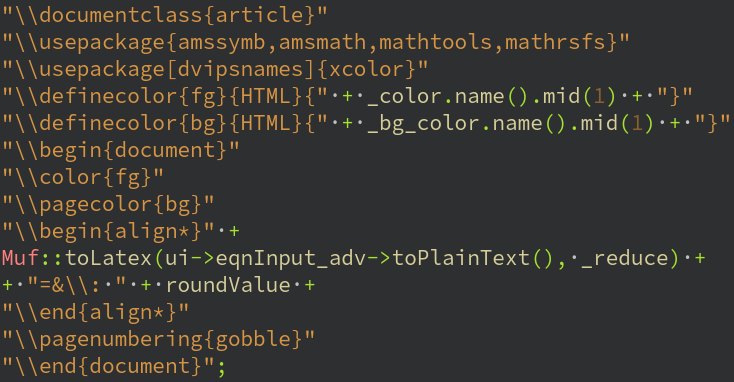
\includegraphics[width=\textwidth]{latex_adv.png}
					\caption{input.latex}
					\label{fig:latex_adv}
				\end{figure}}
			\parbox{\textwidth}{
			\subsubsection{Grafični način}
				V grafičnem načinu funkcija nastavi \textquote{KLFBackend} nastavitve:
				\begin{alignitemize}
					\codequote{input.preamble} &ne nastavi\\
					\codequote{input.mathmode} &ne nastavi\\
					\codequote{input.bypasstemplate} &nastavi na \codequote{true}\\
					\codequote{input.latex} &nastavi tako:
				\end{alignitemize}
				\begin{figure}[H]
					\centering
					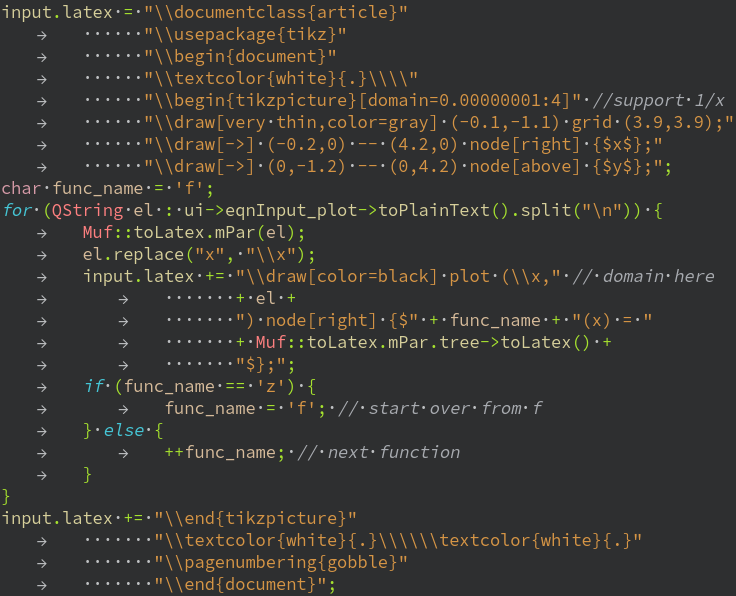
\includegraphics[width=\textwidth]{latex_plot.png}
					\caption{input.latex}
					\label{fig:latex_plot}
				\end{figure}}
	\section{MufExprParser}
		\parbox{\textwidth}{
		Razred \codequote{MufExprParser} v sebi definira več drugih razredov:
		\begin{itemize}
			\item \texttt{enum class Assoc}~(Koda \ref{src:enum_assoc}), ki oštevilči asociativnost operatorja,
			\item \texttt{enum class TokenType}~(Koda \ref{src:enum_tty}), ki oštevilči tip tokena,
			\item \texttt{struct str\_tok\_t}~(Koda \ref{src:str_tok_t}), ki definira token,
			\item \texttt{struct pat\_t}~(Koda \ref{src:pat_t}), ki definira \textquote{regex} vzorec za določen token in
			\item \texttt{class ExprTree}~(Koda \ref{src:exprtree}), ki je implementacija AST.
		\end{itemize}
		}\\
		\begin{spacing}{1}
		\begin{lstlisting}[language=C++, caption=Assoc enum, label=src:enum_assoc]
		enum class Assoc {
			NONE,
			LEFT,
			RIGHT,
			PREFIX,
			POSTFIX
		};
		\end{lstlisting}
		\begin{lstlisting}[language=C++, caption=TokenType enum, label=src:enum_tty]
		enum class TokenType {
			B, // binary op
			b, // brace
			U, // unary
			v, // value
			x, // variable
			NONE
		};
		\end{lstlisting}
		\begin{lstlisting}[language=C++, caption=Razred za hranjenje tokenov, label=src:str_tok_t]
		struct str_tok_t {
			QString         s;
			Assoc           assoc;
			int             prec;
			int             rightPrec;
			int             nextPrec;
			TokenType       type;
			friend bool operator>(const str_tok_t& lhs, const str_tok_t& rhs);
			friend bool operator<(const str_tok_t& lhs, const str_tok_t& rhs);
			friend bool operator>=(const str_tok_t& lhs, const str_tok_t& rhs);
			friend bool operator<=(const str_tok_t& lhs, const str_tok_t& rhs);
			friend bool operator==(const str_tok_t& lhs, const str_tok_t& rhs);
			friend bool operator!=(const str_tok_t& lhs, const str_tok_t& rhs);
		};
		\end{lstlisting}
		\begin{lstlisting}[language=C++, caption=Razred za hranjenje \textquote{regex} vzorea tokena, label=src:pat_t]
		struct pat_t {
			QString         str;
			str_tok_t*      op;
			QRegularExpression re;
		};
		\end{lstlisting}
		\begin{lstlisting}[language=C++, caption=Deklaracija AST, label=src:exprtree]
		class ExprTree
		{
		public:
			ExprTree();
			ExprTree(const ExprTree& rhs);
			ExprTree(str_tok_t v); // set value as operator
			ExprTree(str_tok_t _op, ExprTree _operand);
			ExprTree(str_tok_t _op, ExprTree* _operand);
			ExprTree(str_tok_t _op, ExprTree _left, ExprTree _right);
			ExprTree(str_tok_t _op, ExprTree* _left, ExprTree* _right);
			~ExprTree();
			
			// TODO: add int check
			// check if it's worth to convert
			int             negative();
			// check if it can be reduced to a value
			bool            isValue();
			bool            isFrac();
			bool            hasFrac();
			void            toFrac();
			double          eval();
			bool            isInt();
			bool            isOdd();
			bool            isEven();
			QString         print();
			QString         toLatex();
			void            reduce();
			void            negate();
			void            multiply(const int& factor);
			void            multiply(const QString& var);
			void            multiply(ExprTree* t);
			QStringList     var();
			QString         expr();
			
			str_tok_t       op;    // can be any operator or value
			QList<ExprTree*> operands;
			
		private:
			void            prefixUnary();
			void            setValue(const double& v);
			void            setValue(const QString& v);
			void            setChild(const int& i);
			
		public:
			bool            numeric;
		};
		\end{lstlisting}
		\end{spacing}
		\odstavek
		Razred vsebuje tudi veliko metod, vendar bom napisal le tiste, ki se dejansko uporabljajo.
		Odstranil bom tudi definicije zgoraj navedenih razredov~(Kode:~\ref{src:enum_assoc},~\ref{src:enum_tty},~\ref{src:str_tok_t},~\ref{src:pat_t}~in~\ref{src:exprtree}).
		\begin{spacing}{1}
		\begin{lstlisting}[language=C++, caption=Deklaracija razreda \codequote{MufExprParser}, label=src:mufexprparser]
		class MufExprParser : public QObject
		{
			Q_OBJECT
		public:
			enum class Assoc;
			Q_ENUM(Assoc)
			enum class TokenType;
			Q_ENUM(TokenType)
			struct str_tok_t;
			struct pat_t;
			
			class ExprTree;
			
		public:
			explicit MufExprParser(QObject* parent = nullptr);
			~MufExprParser()
			{
				if (tree != nullptr) {
					delete tree;
					tree = nullptr;
				}
			}
			
		private:
			int             init();
			
			bool            expect(const QString& tok_s); // true if next.s == tok_s
			bool            expect(const str_tok_t& tok); // true if next == tok
			bool            expect(const TokenType& tok_t); // true if next.type == tok_t
			void            consume(); // removes next token
			str_tok_t       next();    // returns next token
			
			bool            tokenize(QString input);
			pat_t*          match(QString s,
			                      QList<pat_t>& p,
			                      str_tok_t* t,
			                      QString* e);
			
			ExprTree*       exprTD(int p);
			ExprTree*       pTD();
			
		public slots:
			QString         exprParseTD(QString input);
		public:
			QString         operator()(QString input);
			
		private:
			// predefined tokens
			static str_tok_t tok_end; // end token
			static str_tok_t op_sent; // sentinel
			static str_tok_t op_rbr;
			static str_tok_t op_lbr;
			static str_tok_t op_exp;
			static str_tok_t op_fac;
			static str_tok_t op_mul;
			static str_tok_t op_div;
			static str_tok_t op_mod;
			static str_tok_t op_add;
			static str_tok_t op_sub;
			static str_tok_t op_equ;
			static str_tok_t op_and;
			static str_tok_t op_or;
			static str_tok_t op_neg;
			static str_tok_t arg_pr;
			static str_tok_t arg_num;
			static str_tok_t arg_var;
			pat_t           pat_eos; // end of string pattern
			QList<pat_t>    pat_ops; // list of operator patterns
			QList<pat_t>    pat_arg; // list of arg? patterns
			
			QQueue<str_tok_t> tokens; // tokens to parse
			QStack<str_tok_t> mOperators;
			QStack<ExprTree> mOperands;
			
		public:
			ExprTree*       tree;
			
			bool            reduce;
			
			friend bool operator>(const str_tok_t& lhs, const str_tok_t& rhs);
		};
		\end{lstlisting}
		\end{spacing}	
		Razred definira tipične metode razredov v C++. To so konstruktor, destruktor, ki sprosti drevo iz spomina, ter metoda \codequote{init}.
		Funkcija se kliče v konstruktorju in inicializira vrednosti spremenljivk.
		Ker so operatorji deklarirani kot statične spremenljivke, jih \codequote{init} skripta ne inicializira, nastavi pa začetne vrednosti članom \angl{member} \codequote{pat\_eos}, \codequote{pat\_ops} in \codequote{pat\_arg}.\odstavek
		Pretvorbo v AST lahko kličemo na dva načina, prvi je metoda \codequote{exprParseTD}, drugi je pa s pomočjo preobloženega operatorja \codequote{()}, kot parameter, jima pa podamo niz z izrazom, ki ga želimo pretvoriti.
		\odstavek
		Razred si definira tudi privatne funkcije, ki olajšajo implementacijo.
		Metoda \codequote{consume} vzame token iz sklada, metoda \codequote{next} pa vrne token na vrhu sklada, če je pa ta prazen pa vrne \codequote{tok\_end}.\odstavek
		\codequote{expect} metode vzamejo neko obliko tokena kot parameter, in če je enak naslednjemu tokenu, le tega vzamejo iz sklada in vrnejo \texttt{true}, drugače pa vrnejo \texttt{false}. \odstavek
		Metoda \codequote{match} glede na \textquote{regex} vzorce izve kakšne vrste token je naslednji v nizu, metoda \codequote{tokenize} pa zaporedno kliče metodo \codequote{match} z različnimi vhodnimi podatki.
		Metodi \codequote{exprTD} in \codequote{pTD} pomagata metodi \codequote{exprParseTD} pri pretvorbi v AST.
\chapter{Navodila za uporabo}
	\section{Jezik kalkulatorja}
		Jezik kalkulatorja je enak jeziku knjižnice Exprtk.
		Te podatke sem preveril na \today, za spremembe pa se nanašajte na uradno dokumentacijo knjižnice.~\cite{exprtk,exprtk_git}
		\begin{alignitemize}
			Osnovni operatorji: &\texttt{+, -, *, /, \%, \^{}} \\
			Prireditev: &\texttt{:=, +=, -=, *=, /=, \%=}\\
			Enakosti in neenakosti: &\texttt{=, ==, <>, !=, <, <=, >, >=}\\
			Logični operatorji: &\group{225pt}{and, mand, mor, nand, nor, not, or, shl, shr, xnor, xor, true, false}\\
			Funkcije: &\group{375pt}{abs, avg, ceil, clamp, equal, erf, erfc, exp, expm1, floor, frac, log, log10, log1p, log2, logn, max, min, mul,  ncdf, nequal, root, round, roundn, sgn, sqrt, sum, swap, trunc}\\
			Trigonometrija: &\group{330pt}{acos, acosh, asin, asinh, atan, atanh, atan2, cos, cosh, cot, csc, sec, sin, sinc, sinh, tan, tanh, hypot, rad2deg, deg2grad, deg2rad, grad2deg}\\
			Nadzor pretoka: &\group{250pt}{if-then-else, trojiški pogojni operator~(?:), switch-case, return}\\
			Zanke: &\texttt{while, for, repeat-until, break, continue}
		\end{alignitemize}
		Različni stavki so ločeni s podpičjem (\texttt{;}), kalkulator bo pa izpisal vrednost zadnjega izraza.\odstavek
		Aplikacija podpira tudi definicijo funkcij, ki se naložijo ob zagonu programa.
		Definicije funkcij se nahajajo v mapi \textquote{function}.
		V tej mapi so funkcije razdeljene na \textquote{skupine} predstavljene s podmapami.
		Na primer funkcija \codequote{add} se nahaja v datoteki \textquote{math} v mapi \textquote{stl}, torej lahko rečemo da pripada knjižnici \textquote{math} iz skupine \textquote{stl}.
		Imena funkcij se ne smejo ponavljati.
		\odstavek
		Aplikacija v večini primerov spremenljivke obravnava kot globalne spremenljivke. Uporabnik jih preprosto inicializira \codequote{x := 3} (ali doda z uporabniškim vmesnikom) in potem jih lahko prosto uporablja.
		Na voljo so pa tudi lokalne spremenljivke, ki se uporabljajo, ko v izrazu ni nobenih zunanjih (globalnih) spremenljivk, vendar so vse uporabljene spremenljivke definirane v izrazu. V tem primeru \emph{moramo} uporabiti rezervirano besedo \codequote{var}. 
		\begin{spacing}{0.15}
		\parbox{\textwidth}{Nekaj primerov preprostih izrazov, ki uporabljajo le lokalne spremenljivke so:\\
		\begin{itemize}
			\item \texttt{1 + 2}
			\item \texttt{var x := 3; 2 * x - 3}
			\item \texttt{var x := 3; var y := abs(x - 8); x - y / 7}
		\end{itemize}}
		\end{spacing}
		\begin{spacing}{1.5}
			\wdot
		\end{spacing}
		\parbox{\textwidth}{\begin{spacing}{0}
		Sintaksa kontrolnih struktur je zelo podobna C, C++ ipd.:
		\begin{itemize}
			\item \parbox{\textwidth}{\vspace{5px}\setstretch{0.8}\texttt{if(cond) \{\\\wdot\qquad expr1;\\ \wdot\qquad expr2;\\\};}\vspace{5px}}
			\item \parbox{\textwidth}{\vspace{5px}\setstretch{0.8}\texttt{if(cond) \{\\\wdot\qquad expr1;\\ \wdot\qquad expr2;\\\} else \{\\\wdot\qquad expr3;\\ \wdot\qquad expr4;\\\};}\vspace{5px}}
			\item \parbox{\textwidth}{\vspace{5px}\setstretch{0.8}\texttt{switch \{\\\wdot\qquad case cond: expr1;\\ \wdot\qquad case cond: expr2;\\\};}\vspace{5px}}
			\item \parbox{\textwidth}{\vspace{5px}\setstretch{0.8}\texttt{while(cond) \{\\\wdot\qquad expr1;\\ \wdot\qquad expr2;\\\};}\vspace{5px}}
			\item \parbox{\textwidth}{\vspace{5px}\setstretch{0.8}\texttt{repeat \\\wdot\qquad expr1;\\ \wdot\qquad expr2;\\ untill(cond);}\vspace{5px}}
			\item \parbox{\textwidth}{\vspace{5px}\setstretch{0.8}\texttt{for(init;cond;iter) \{\\\wdot\qquad expr1;\\ \wdot\qquad expr2;\\\};}\vspace{5px}}
			\item \texttt{break} in \texttt{break[]} zapusti zanko in vrne vrednost znotraj \texttt{[]}.
			\item \texttt{continue} spusti iteracijo in nadaljuje z izvajanjem zanke
			\item Trojiški operator: cond ? exprT : exprF
			\item \texttt{~(expr1, expr2) == expr2}:\\
			Izračuna vse pod-izraze potem pa vrne zadnji pod-izraz.
			\item \parbox{\textwidth}{\vspace{5px}\setstretch{0.8}\texttt{[*] \{\\\wdot\qquad case cond: expr1;\\ \wdot\qquad case cond: expr2;\\\};}\vspace{5px}}
			Za razliko od \texttt{switch-case} bo \texttt{[*]} izračunal vse izraze za katere je \texttt{cond} enak \texttt{true}
		\end{itemize}
		\end{spacing}}
		\subsection{Vhodno/izhodne operacije}
			Exprtk pozna dve vrsti I/O operacij (vhodno/izhodnih, iz angl. Input/Output):
			\begin{itemize}
				\item Standardne vhodno/izhodne operacije:
				\begin{enumerate}
					\item \texttt{print}
					\item \texttt{println}
				\end{enumerate}
				\item Datotečne vhodno/izhodne operacije:
				\begin{multicols}{3}
				\begin{enumerate}
					\item \texttt{open}
					\item \texttt{close}
					\item \texttt{write}
					\item \texttt{read}
					\item \texttt{getline}
					\item \texttt{eof}
				\end{enumerate}
				\end{multicols}
			\end{itemize}
		\subsection{Vektorske operacije}
			%TODO: basic vectors
			Na voljo so tudi dodatne vektorske funkcije:
			\begin{multicols}{3}
			\begin{enumerate}
				\item \texttt{all\_true}
				\item \texttt{all\_false}
				\item \texttt{any\_true}
				\item \texttt{any\_false}
				\item \texttt{count}
				\item \texttt{copy}
				\item \texttt{rotate-left}
				\item \texttt{rotate-right}
				\item \texttt{shift-left}
				\item \texttt{shift-right}
				\item \texttt{sort}
				\item \texttt{nth\_element}
				\item \texttt{iota}
				\item \texttt{sumk}
				\item \texttt{axpy}
				\item \texttt{axpby}
				\item \texttt{axpyz}
				\item \texttt{axpbyz}
				\item \texttt{axpbyz}
				\item \texttt{dot}
				\item \texttt{dotk}
			\end{enumerate}
			\end{multicols}
			
\chapter{Zaključek}
	Med izdelavo aplikacije sem se naučil veliko o orodjih, ki sem jih uporabljal, pridobil sem znanje \LaTeX-a, poglobil sem znanje o avtomatskih sistemih za gradnjo projektov kot so  \textquote{qmake} in \textquote{CMake}, pridobil sem pa tudi veliko pomembnih izkušenj, na primer z uporabo \textquote{GitHub}-a za nadziranje verzij programa in z uporabo \LaTeX-a v programu za izrisovanje računov, pa tudi za pisanje tega poročila.\odstavek
	Iz izobraževalnega vidika, sem verjetno največ pridobil z implementacijo TRS in SRS ter z implementacijo razčlenjevanja \angl{parsing}, saj so to dokaj napredne teme, in jih je težko implementirati v tako nizko-nivojskem jeziku kot je C++.\odstavek
	Dobil sem malo izkušenj tudi s pisanjem knjižnic, ko sem pisal alternativo Qt razredu \codequote{QTranslate}.\odstavek
	Programu trenutno manjka stabilnost, saj ni čudno, če se sesuje ko mu podamo čuden vhod, in samostojnost, saj se zanaša na zunanje programe za prevajanje \LaTeX{} kode. Izboljšati bi se tudi dalo grafični način, saj trenutno izrisuje samo na definicijskem območju $x \in (0, 4]$ in ne bo izrisal ničesar, če katera od funkcij tam ni definirana, tako da je bolj \textquote{proof-of-concept} kot pa dejansko uporabna funkcionalnost aplikacije. \odstavek
	Čeprav sem nameraval narediti bolj zmogljiv kalkulator, ki bi reševal enačbe, se je izkazalo, da nimam več let in skupine doktorjev znanosti, tako da sem kar zadovoljen s funkcijami, ki mi jih je uspelo implementirati.

%\chapter{Viri in literatura}
%{qt docs}\\
%{tex.stackexchange}\\
%{stackoverflow.net}\\
%{exprtk pages}\\

\newpage
\chapter{Viri}
\printbibliography[heading=none]
\texttt{https://stackoverflow.com/}\\
\texttt{https://tex.stackexchange.com/}
\section{Viri slik}
\texttt{http://www.ecma-international.org/publications/files/ECMA-ST/ECMA-404.pdf}
\newpage
\pagestyle{empty}
\subsection*{Izjava o avtorstvu}
Izjavljam, da je strokovno poročilo Kalkulator v celoti moje avtorsko delo, ki sem ga izdelal samostojno s pomočjo navedene literature in pod vodstvom mentorja.\\[5cm]
Ljubljana, \today \hfill Rok Strah

\end{document}


























































